\documentclass[12pt]{beamer}
\usepackage[utf8]{inputenc}
\usepackage[T1]{fontenc}
\usepackage{amsmath}
\usepackage{amsfonts}
\usepackage{amssymb}
\usepackage{graphicx}
\usepackage{bussproofs}
\usepackage{lmodern}
\newenvironment{boxedprooftree}[1][c]
 {\begin{tabular}[#1]{@{}c@{}}}
 {\DisplayProof\end{tabular}}
 
\usetheme{Copenhagen}
\usepackage{listings}

\lstdefinelanguage{JavaScript}{
  keywords={const, let, break, case, catch, continue, debugger, default, delete, do, else, finally, for, function, if, in, instanceof, new, return, switch, this, throw, try, typeof, var, void, while, with, class, constructor, public, private, boolean, string, number, export,yield, any, true, false, undefined, null},
  morecomment=[l]{//},
  morecomment=[s]{/*}{*/},
  morestring=[b]',
  morestring=[b]",
  sensitive=true
}

\lstset{
   language=JavaScript,
   showstringspaces=false,
   basicstyle=\tiny,
   showspaces=false,
   tabsize=2,
   escapechar={^}
}
\AtBeginSection[]
{
  \begin{frame}
    \frametitle{Table of Contents}
    \tableofcontents[currentsection]
  \end{frame}
}
\begin{document}
\newcommand{\mathsc}[1]{{\normalfont\textsc{#1}}}
\newcommand{\tforce}[2]{\mathfrak{V}\left(#1, #2\right)}
%\newcommand{thunk}[2]{\mathbb{T}\left(#1,#2\right)}
\author{Ian Duncan and Ahmed Jellouli}
\title{Lazy Evaluation for Source}
%\subtitle{}
%\logo{}
%\institute{}
\date{CS4215 Final Project, 13 April 2020}
%\subject{Hi}
%\setbeamercovered{transparent}
\setbeamertemplate{navigation symbols}{}
\begin{frame}[plain]
	\maketitle
\end{frame}

\begin{frame}
\frametitle{Table of Contents}
\tableofcontents
\end{frame}

\section{Introduction}

\begin{frame}
\frametitle{Evaluation Strategies}
\begin{itemize}
\item<1->In \textbf{call-by-value} or \textbf{strict} evaluation, all arguments to a function are evaluated at application time.

\item<2->In \textbf{call-by-name} evaluation, arguments to a function are evaluated each time they are needed.

\item<3->In \textbf{call-by-need} or \textbf{lazy} evaluation, arguments to a function are evaluated the first time they are needed. The result of this evaluation is memoized in case the argument is needed again.
\end{itemize}
\end{frame}

\begin{frame}
\frametitle{Project Goals}
We aimed to produce a lazy version of Source\S2, which entailed the following deliverables:\pause
\begin{enumerate}
\item<2->A specification for ``Lazy Source'' 
\item<3->A metacircular evaluator
\item<4->Support for lazy evaluation in the interpreter and transpiler of \texttt{js-slang}
\item<5->Integration into Source Academy frontend
\item<6->Example programs
\item<7->Documentation
\end{enumerate}
\end{frame}

\section{Specification}

\begin{frame}
\frametitle{Inspiration}
Our specification follows the presentation of lazy evaluation in SICPJS\S4.2:\pause[1]
\begin{itemize}
\item<2->Application of user-defined functions is non-strict
\item<3->Application of built-ins (except for \texttt{pair} to support lazy lists), including binary operators is strict
\item<4->Evaluation of name bindings is strict
\end{itemize}
\pause[5]Note that this specification differs from Haskell, where \textit{all} of these are non-strict.
\end{frame}

\begin{frame}
\frametitle{Denotational Semantics of Delayed Computations}
\begin{itemize}
\item<1-> We introduce the concept of a \textbf{thunk}, which is an unevaluated expression and its associated environment, to support delayed evaluation of arguments.
\item<2-> In our denotation semantics, given an expression $E$ and associated environment $\Delta$, we represent the thunk of $E$ and $\Delta$ as $\theta(\Delta, E)$.
\item<3-> Thunks can be \textbf{forced} as needed to yield a ``final result'' of evaluating an $E$ with respect to $\Delta$ that is not a thunk.
\end{itemize}
\end{frame}

\begin{frame}
\frametitle{Denotational Semantics of Forcing Thunks}
Let $\mathbb{T}$ be the set of all thunks. Then, define the function $\mathfrak{F}:\mathbb{T}\to\textbf{EV}$ by
\[ \mathfrak{F}\left(\theta(\Delta, E)\right) = \begin{cases} 
      v & v\notin\mathbb{T} \\
      \mathfrak{F}(v) & \text{otherwise},
   \end{cases}
\]
where $\Delta\Vdash E \rightarrowtail v$.



\end{frame}

\begin{frame}
\frametitle{Denotational Semantics of Forcing Expressions}
Define the function $\mathfrak{V}:\textbf{Env}\times\textbf{S2}\to\mathbf{EV}$ by
\[ \mathfrak{V}\left(\Delta,E\right) = \begin{cases} 
      v & v\notin\mathbb{T} \\
      \mathfrak{F}(v) & \text{otherwise},
   \end{cases}
\]
where $\Delta\Vdash E \rightarrowtail v$.\pause

\vspace{1em}We use $\mathfrak{V}$ instead of $\cdot\Vdash\cdot\rightarrowtail$ to evaluate entire programs, because we do not want the final result to be a thunk.
\end{frame}

\begin{frame}
\frametitle{Denotational Semantics of Application}
In Lazy Source, we say that a function $f$ is \textbf{strict} if it is built-in (except for \texttt{pair}), and \textbf{non-strict} otherwise.\pause
\[
\begin{tabular}{@{} l c @{}}
[\textsc{SApp}] &
  \begin{boxedprooftree}
  \AxiomC{$\tforce{\Delta}{E_1}=f$}
  \AxiomC{$\tforce{\Delta}{E_2}=v_2,\ldots,\tforce{\Delta}{E_n}=v_n$}
  \BinaryInfC{$\Delta\Vdash E_1(E_2,\ldots,E_n)\rightarrowtail f(v_2,\ldots,v_n)$}
  \end{boxedprooftree}
\end{tabular}
\]
where $f$ is \textbf{strict}.\pause
\[
\begin{tabular}{@{} l c @{}}
[\textsc{NSApp}] &
  \begin{boxedprooftree}
  \AxiomC{$\tforce{\Delta}{E_1}=f$}
  \AxiomC{$E_2,\ldots,E_n$}
  \BinaryInfC{$\Delta\Vdash E_1(E_2,\ldots,E_n)\rightarrowtail f(\theta(\Delta, E_2),\ldots,\theta(\Delta, E_n))$}
  \end{boxedprooftree}
\end{tabular}
\]
where $f$ is \textbf{non-strict}.
\end{frame}

\begin{frame}
\frametitle{Denotational Semantics of Operators}
Binary and unary operators always force their arguments:
\[
\begin{tabular}{@{} l c @{}}
[\textsc{BinOp}] &
  \begin{boxedprooftree}
  \AxiomC{$\tforce{\Delta}{E_1}=v_1$}
  \AxiomC{$\tforce{\Delta}{E_2}=v_2$}
  \BinaryInfC{$\Delta\Vdash E_1\cdot E_2\rightarrowtail v_1 \cdot v_2$}
  \end{boxedprooftree}
\end{tabular}
\]
where $\cdot\in\{+,*,-,/,\%,\&\&,||\,>,<,>=,<=,== =,!==\}$.
\[
\begin{tabular}{@{} l c @{}}
[\textsc{UnOp}] &
  \begin{boxedprooftree}
  \AxiomC{$\tforce{\Delta}{E}=v$}
  \AxiomC{}
  \BinaryInfC{$\Delta\Vdash \$E\rightarrowtail \$v$}
  \end{boxedprooftree}
\end{tabular}
\]
where $\$\in\{!,-\}$.
\end{frame}

\begin{frame}
\frametitle{Denotational Semantics of Conditional Expressions}
Conditional expressions force their conditions:
\[
\begin{tabular}{@{} l c @{}}
[\textsc{CondTrue}] &
  \begin{boxedprooftree}
  \AxiomC{$\tforce{\Delta}{E_1}=\texttt{true}$}
  \AxiomC{$\Delta\Vdash E_2\rightarrowtail v_2$}
  \BinaryInfC{$\Delta\Vdash E_1\text{ }?\text{ }E_2 : E_3\rightarrowtail v_2$}
  \end{boxedprooftree}
\end{tabular}
\]
\[
\begin{tabular}{@{} l c @{}}
[\textsc{CondFalse}] &
  \begin{boxedprooftree}
  \AxiomC{$\tforce{\Delta}{E_1}=\texttt{false}$}
  \AxiomC{$\Delta\Vdash E_3\rightarrowtail v_3$}
  \BinaryInfC{$\Delta\Vdash E_1\text{ }?\text{ }E_2 : E_3\rightarrowtail v_3$}
  \end{boxedprooftree}
\end{tabular}
\]
\end{frame}

\section{Metacircular Evaluator}
\begin{frame}[fragile]
\frametitle{Representing Thunks}
We represent thunks as tagged lists:
\begin{lstlisting}[language=JavaScript]
function delay_it(exp, env) {
    return list("thunk", exp, env);
}

function thunk_exp(thunk) {
    return head(tail(thunk));
}

function thunk_env(thunk) {
    return head(tail(tail(thunk)));
}
\end{lstlisting}
\end{frame}

\begin{frame}[fragile]
\frametitle{Forcing Thunks}
To get the actual value of evaluating an expression (i.e., not a thunk), we define an \texttt{actual\_value} function:
\begin{lstlisting}
function actual_value(exp, env) {
    return force_it(evaluate(exp, env));
}
\end{lstlisting}
\end{frame}

\begin{frame}[fragile]
\frametitle{Forcing Thunks}
The function \texttt{force\_it} is mutually recursive with \texttt{actual\_value}, and handles memoization:
\begin{lstlisting}
function force_it(obj) {
    if(is_thunk(obj)) {        
        const result = actual_value(thunk_exp(obj), thunk_env(obj));        
        set_head(obj, "evaluated_thunk");
        set_head(tail(obj), result);
        set_tail(tail(obj), null);        
        return result;        
    } else if(is_evaluated_thunk(obj)) {        
        return thunk_value(obj);        
    } else {
        return obj;
    }    
}
\end{lstlisting}
\end{frame}

\begin{frame}[fragile]
\frametitle{Function Application}
We define two functions to help us delay or force function arguments as needed:
\begin{lstlisting}
function list_of_arg_values(exps, env) {
    return no_operands(exps)
        ? null
        : pair(actual_value(first_operand(exps), env),
          list_of_arg_values(rest_operands(exps), env));
}

function list_of_delayed_args(exps, env) {
    return no_operands(exps)
        ? null
        : pair(delay_it(first_operand(exps), env),
          list_of_delayed_args(rest_operands(exps), env));
}
\end{lstlisting}
\end{frame}

\begin{frame}[fragile]
\frametitle{Function Application}
Then we modify \texttt{apply} to delay or force arguments as needed:
\begin{lstlisting}
function apply(fun, args, env) {
    if (is_primitive_function(fun)) {
      return apply_primitive_function(fun, list_of_arg_values(args,env));
   } else if (is_compound_function(fun)) {
      ...
      const delayed_args = list_of_delayed_args(args, env);
      const values = append(delayed_args, temp_values);			   
      const result =
         evaluate(body,
                  extend_environment(
                      names,
                      values,
                      function_environment(fun)));
      ...
   }
   ...
}
\end{lstlisting}
\end{frame}

\begin{frame}[fragile]
\frametitle{Lazy Lists}
We implement lazy lists in the metacircular evaluator by:
\begin{itemize}
\item<1->making  \texttt{pair}, \texttt{head} and \texttt{tail} primitive operators of the language. 
\item<2->evaluating \texttt{pair} as a ``special case'', whereby the evaluation is lazy and the arguments are not forced.
\item<3->Arguments of \texttt{head} and \texttt{tail} need to be forced because we make use of the underlying source implementation.
\end{itemize}
\end{frame}

\begin{frame}[fragile]
\frametitle{Evaluate}
Finally, we make a small change to the \texttt{evaluate} function to let \texttt{apply} have full control in handling function arguments. We also force thunks as needed (e.g., at the top level and in conditional expressions):
\begin{lstlisting}
function evaluate(stmt, env) {
   return is_self_evaluating(stmt)
          ?  stmt
        ...
        : is_application(stmt)
          ? is_pair_constructor(stmt) ? construct_lazy_pair(operands(stmt),env) 
           : apply(actual_value(operator(stmt), env),
                  operands(stmt), env)
        ...
}

function eval_toplevel(stmt) {
   const program_block = make_block(stmt);
   const value = actual_value(program_block, 
                          the_global_environment);
   ...
}
\end{lstlisting}
\end{frame}

\section{Implementation in \texttt{js-slang}}

\subsection{Overview}

\begin{frame}
\frametitle{Overview}
\begin{itemize}
\item<1-> We modify the interpreter and transpiler of \texttt{js-slang} to support lazy evaluation, if explicitly enabled.
\item<2-> The evaluation method (strict or lazy) is controlled by a \texttt{variant} property of the execution context.
\item<3-> The implementation of the interpreter mirrors that of the metacircular evaluator.
\item<4-> We modify the transpiler to thunk arguments in transpiled code if lazy evaluation is enabled, and alter native runtime operators to handle thunks if they are present.
\end{itemize}
\end{frame}

\subsection{Transpiler}

\begin{frame}[fragile]
\frametitle{Representing Thunks in Transpiled Code}
\begin{itemize}
\item<1-> Delaying a computation $E$ is as simple as making $E$ the body of a nullary arrow function: \texttt{() => E}

\item<2-> Since we also want to memoize our thunks, we create an object instead:
\begin{lstlisting}
{isThunk: true, expr: () => E, memoizedValue: 0, isMemoized: false}
\end{lstlisting}
\end{itemize}
\end{frame}

\begin{frame}
\frametitle{Creating Thunks at Compile Time}
\begin{itemize}
\item<1-> Function calls in Source are wrapped with a call to the native runtime operator \texttt{callIfFuncAndRightArgs}. For example, \texttt{f(a, b, c)} is transformed to \texttt{callIfFuncAndRightArgs(f, lineno, colno, a, b, c)}.
\item<2-> If lazy evaluation is enabled, we also thunk the arguments during this transformation. So, \texttt{f(a, b, c)} is transformed to \texttt{callIfFuncAndRightArgs(f, lineno, colno, \{expr: () => a, ...\}, ...)}
\item<3-> We alter the transformation \texttt{transformReturnStatementsToAllowProperTailCalls} in a similar way.
\end{itemize}
\end{frame}

\begin{frame}[fragile]
\frametitle{Handling Thunks at Runtime}
We define a new native runtime operator \texttt{forceIt} to force thunks when needed:
\begin{lstlisting}
export function forceIt(val: any): any {
  if (val !== undefined && val !== null && val.isThunk === true) {
    if (val.isMemoized) {
      return val.memoizedValue
    }
    const evaluatedValue = forceIt(val.expr())
    val.isMemoized = true
    val.memoizedValue = evaluatedValue
    return evaluatedValue
  } else {
    return val
  }
}
\end{lstlisting}
\end{frame}

\begin{frame}[fragile]
\frametitle{Handling Thunks at Runtime}
We then modify \texttt{callIfFuncAndRightArgs} to force thunks when necessary:
\begin{lstlisting}
export function callIfFuncAndRightArgs(candidate: any, line: number, column: number, 
                ...args: any[])
{
  ...
  candidate = forceIt(candidate)
  if (typeof candidate === 'function') {
    if (candidate.transformedFunction === undefined) {
      try {
        const forcedArgs = args.map(forceIt)
        return candidate(...forcedArgs)
      } catch (error) {
        ...
      }
    } else {
      ...
      return candidate(...args)
    }
  } else {
    ...
  }
}
\end{lstlisting}
\end{frame}

\begin{frame}
\frametitle{Handling Thunks at Runtime}
\begin{itemize}
\item<1-> We also make sure to force thunks in the native runtime operators \texttt{boolOrErr}, \texttt{unaryOp}, and \texttt{binaryOp} using \texttt{forceIt}.
\item<2-> Finally, we apply \texttt{forceIt} to the last statement in the program so that the final result of program evaluation is not a thunk.
\end{itemize}
\end{frame}

\subsection{Lazy Lists}

\begin{frame}
\begin{itemize}
\item<1->\frametitle{Lazy Lists}
Primitive list constructors: \texttt{pair} and \texttt{list} are are now wrapped by an object definition \texttt{LazyBuiltIn} in order to indicate that their arguments need to be thunked.
\item<2-> \texttt{head}, \texttt{tail}, \texttt{is\_pair} and \texttt{is\_null} can remain as the usual primitive functions as we need to force their arguments.
\item<3->Note that this implies that not even \texttt{head} or \texttt{tail} will force elements of the list; they will return the corresponding thunks instead. 
\item<4->We modify the interpreter and the transpiler accordingly to deal with the case of applying \texttt{LazyBuiltIn} instances.
\end{itemize}
\end{frame}

\begin{frame}[fragile]
\frametitle{List standard library}
\begin{itemize}
\item<1->The list "prelude" functions need to be slightly modified in order to stay consistent with the non lazy lists, specifically in error handling. For example, the implementation of \texttt{list\_ref}:
\begin{lstlisting}
function list_ref(xs, n) {
  return n === 0 ? head(xs) : list_ref(tail(xs), n - 1);
}
\end{lstlisting}
leads to an infinite loop is n is negative, because the \texttt{tail(xs)} call is never evaluated.
Instead force its evaluation:

\end{itemize}
\end{frame}

\begin{frame}[fragile]
\frametitle{List standard library}
\begin{lstlisting}
function list_ref(xs, n) {
  const rest = tail(xs);
  return n === 0 ? head(xs) : list_ref(rest, n - 1);
}
\end{lstlisting}
\begin{itemize}
    \item <1-> A similar modification is needed for \texttt{enum\_list}.
    \item <2-> Aim was to stay consistent with non lazy lists behaviour. 
\end{itemize}
\end{frame}

\begin{frame}
\frametitle{Some interesting problems going forward}
\begin{itemize}
    \item lazy list allow us to create seemingly "infinite" streams, e.g: \texttt{const a = pair(1,a);} creates an infinite lists of ones.
    \item <2-> This introduces problems for functions like \texttt{equal, remove\_all, member, filter} which can run into infinite recursion, and \texttt{reverse} which should simply not be usable on infinite lists.
    \item<3-> The question is then whether we could modify these functions so that, for e.g \break \texttt{const a = pair (1,a); remove\_all(1,a);} would evaluate to \texttt{null.}
\end{itemize}
\end{frame}

\begin{frame}
\frametitle{Some interesting problems going forward}
\begin{itemize}
    \item<1-> or : \break
    \texttt{const a = pair(1,a); \break const b = pair (1,b); \break equal(a,b);} evaluates to \texttt{true.}
    \item<2-> Most likely not possible in the general case but might be done if the list is cyclic. Idea is to detect cycles in the list and operate on these finite portions. 
\end{itemize}
\end{frame}




\subsection{Testing}

\begin{frame}[fragile]
\frametitle{Testing}
\begin{itemize}
\item<1-> We implement unit tests to show that the interpreter and transpiler both follow our specification for lazy evaluation.
\item<2-> We test memoization of thunks by making explicit use of side-effects:
\begin{lstlisting}
let x = 1;
function incX() {
  x = x + 1;
  return x;
}
function square(n) {
  return n * n;
}
square(incX()); // should evaluate to 4
\end{lstlisting}
\end{itemize}
\end{frame}

\section{Source Academy Frontend}

\begin{frame}
\frametitle{Source Academy Frontend}
We build on the work of Anubhav and Arsalan to add lazy variants of Source\S1 and Source\S2 to Source Academy:
\begin{center}
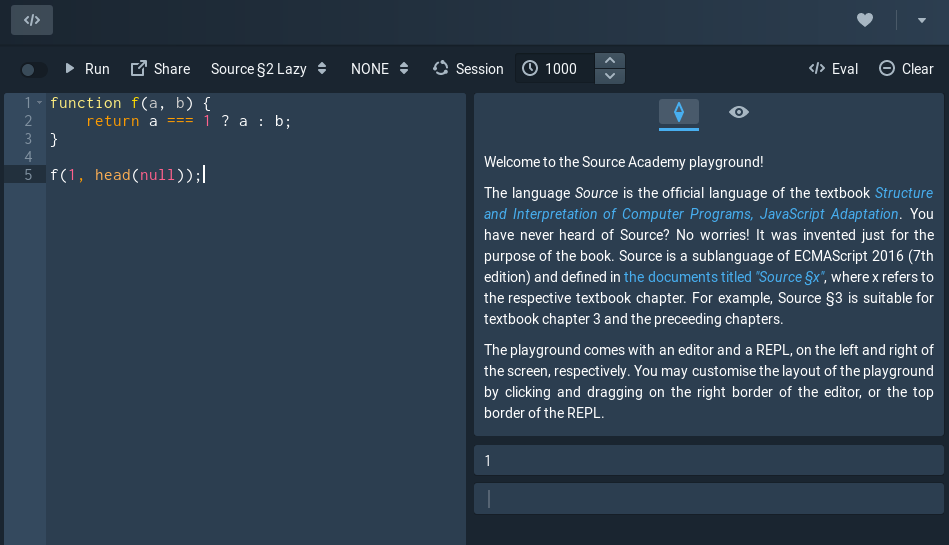
\includegraphics[width=0.7\linewidth]{safrontend}
\end{center}
\end{frame}

\section{Example Programs}


\subsection{A List of all Factorial Numbers}

\begin{frame}
\frametitle{A Recursive Definition of Factorial}
Consider the following recursive definition of the factorial function:
\begin{align*}
0! &= 1 \\
(n+1)! &= (n+1)\times n!
\end{align*}
\end{frame}

\begin{frame}[fragile]
\frametitle{Combining Lists with \texttt{zipWith}}
We can combine the elements of two lists \texttt{xs} and \texttt{ys} into a single list with an additional function \texttt{f} using the operation \texttt{zipWith}:
\begin{lstlisting}
function zipWith(f, xs, ys) {
	return is_null(xs)
		? null
		: is_null(ys)
		? null
		: pair(f(head(xs), head(ys)), zipWith(f, tail(xs), tail(ys)))
}
\end{lstlisting}
\end{frame}

\begin{frame}[fragile]
\frametitle{A List of all Integers from $n$}
We can compute an infinite list of all integers from $n$:
\begin{lstlisting}
function intsFrom(n) {
	return pair(n, intsFrom(n+1));
}
\end{lstlisting}
\end{frame}

\begin{frame}[fragile]
\frametitle{Putting it all Together}
We can use \texttt{zipWith} and \texttt{intsFrom} to compute an infinite list of all factorials $0!, 1!, 2!,\ldots$:
\begin{lstlisting}
const factorials = pair(1, zipWith((x, y) => x*y, intsFrom(1), factorials));
\end{lstlisting}\pause
Conceptually, \texttt{factorials} is the list
\begin{align*}
1 &:: 1 \times 0! :: 2 \times 1! :: 3 \times 2! :: \cdots \\
0! &:: 1! :: 2! :: 3! :: \cdots
\end{align*}
To compute $n!$, just find the $n$th element of \texttt{factorials}.
\end{frame}

\subsection{Generating prime numbers using the Sieve of Eratosthenes}

\begin{frame}
\frametitle{Algorithm}
\begin{itemize}
    \item start with all the natural numbers from 2.
    \item 2 is a prime number, remove all multiples of two from the list.
    \item next item in the list is 3, remove all multiples of 3.
    \item etc..
\end{itemize}

\end{frame}

\begin{frame}[fragile]
\frametitle{Very easy to implement using lazy lists!}

\begin {lstlisting}
function sieve (l) { 
          return pair(head(a), filter (y => y % head(a) !== 0,tail(a)); }
const primes = sieve(intsFrom(2));}
\end{lstlisting}

\end{frame}
\end{document}

